\documentclass[11pt,a4paper,titlepage]{article}
\usepackage[utf8x]{inputenc}
\usepackage{ucs}
\usepackage{ulem}
\usepackage{amsmath}
\usepackage{amsfonts}
\usepackage{amssymb}
\usepackage{pdfpages}
\usepackage[linkbordercolor={1 1 1}, urlbordercolor={1 1 1}]{hyperref}
\usepackage[german]{babel}
\usepackage{eurosym}
\usepackage{pdfpages}
\usepackage{graphicx}
\usepackage{float}
\setcounter{secnumdepth}{4} 
\setlength{\parindent}{3em}
\usepackage[paper=a4paper,left=15mm,right=15mm,top=20mm,bottom=20mm]{geometry}
\pagestyle{plain} 
\title{{\Huge Versionshinweise} \linebreak \linebreak

\includegraphics[width= 35px]{BilderHandbuch/icon32.png} \\
\textbf{Testsuite-Management}
\linebreak \linebreak Änderungen in Version 1.5.2}
\usepackage[space,extendedchars]{grffile}
\begin{document}

\maketitle
\pagebreak

\tableofcontents
\pagebreak

\section{Einleitung}
\subsection{Inhalt}
Dieses Dokument beschreibt die Änderungen an TSM von Version 1.5.1 zu Version 1.5.2.

\subsection{Konvention}
Benutzerelemente und Oberflächenelemente die ausgewählt werden, sind in \texttt{Schreibmaschinenschrift} dargestellt.

\section{Änderungen an der Benutzeroberfläche}
\subsection{Selektiver Export nach Status und Priorität und Überblick über die Entwicklung eines einzelnen Testfalls}
 \begin{figure}[H]
 \centering
 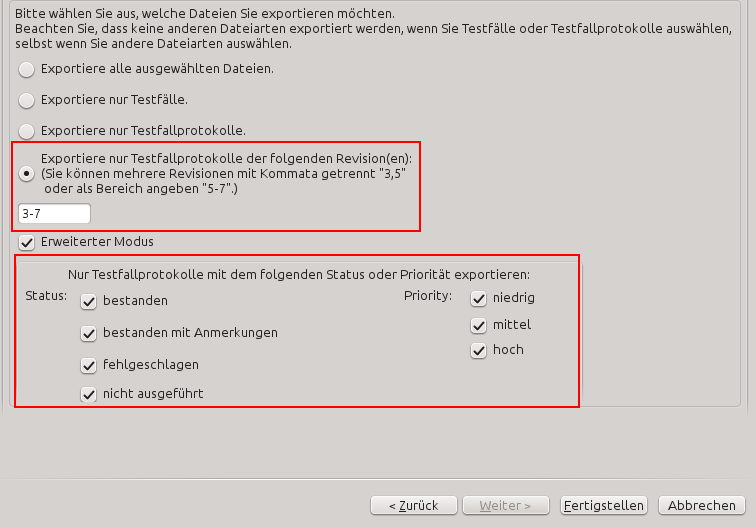
\includegraphics[width=\textwidth]{./BilderAenderungen/pdf-export.png}
 % pdf-export.png: 768x1012 pixel, 101dpi, 19.32x25.45 cm, bb=0 0 548 721
\end{figure}
Der Export von Daten in PDF-Dateien kann nun individueller erfolgen.
So ist es nun möglich, nach Status und Priorität zu filtern sowie einzelne Revisionen oder ganze Revisionsbereiche auszuwählen.


\subsection{Dokumentation früherer Versionsstände eines Testfalls}
\begin{figure}[H]
 \centering
 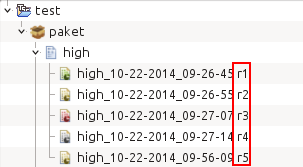
\includegraphics[width=\textwidth]{./BilderAenderungen/revisionsnummer-navigator.png}
 % revisionsnummer-navigator.png: 303x167 pixel, 101dpi, 7.62x4.20 cm, bb=0 0 216 119
\end{figure}
Im Navigator werden die Revisionsnummern der Testfallprotokolle deutlicher hinter dem Dateinamen angezeigt.

\subsection{Versionsfeld}
\begin{figure}[H]
\centering
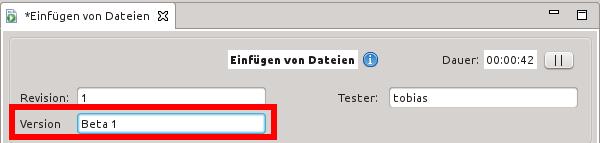
\includegraphics[width=\textwidth]{./BilderAenderungen/versionsfeld.png}
% versionsfeld.png: 1183x150 pixel, 101dpi, 29.75x3.77 cm, bb=0 0 843 107
\end{figure}
Bei der Testfallausführung kann nun zusätzlich zur Revisionsnummer eine Versionsbezeichnung als Freitext eingegeben werden.

\subsection{Eindeutigere Bezeichnung für "`Dauer"'}
\begin{figure}[H]
 \centering
 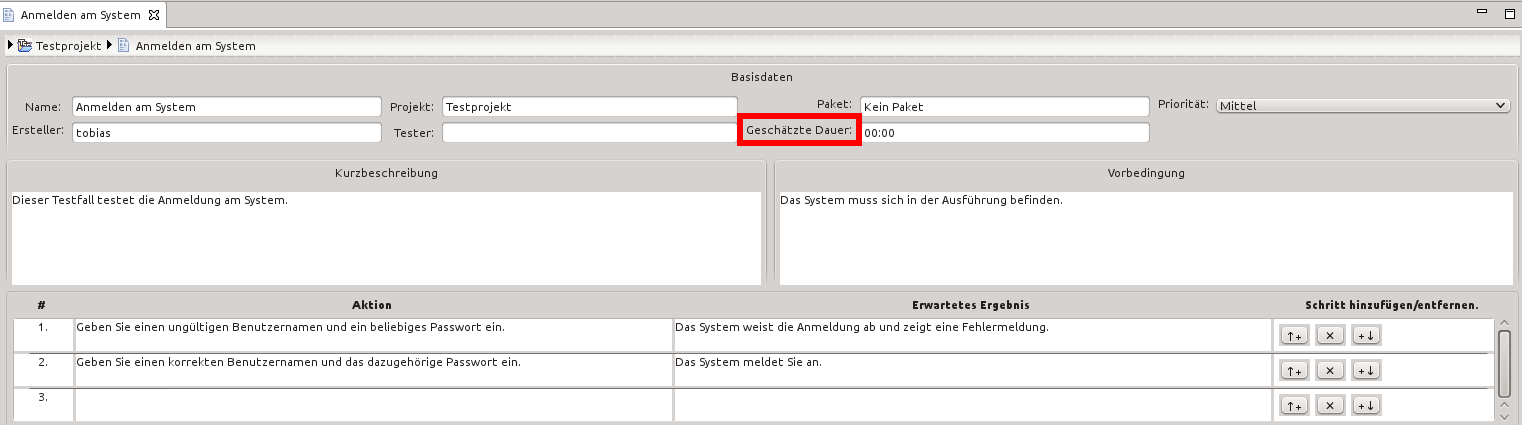
\includegraphics[scale=0.6]{./BilderAenderungen/testfall-bearbeiten-dauer-neu.png}
 % testfall-bearbeiten-dauer.png: 1183x424 pixel, 96dpi, 31.30x11.22 cm, bb=0 0 887 318
\end{figure}
Beim Bearbeiten eines Testfalls ist das Feld "`Dauer"' in "`Geschätzte Dauer"' umbenannt worden, um dessen Funktion deutlicher zu machen.

\subsection{Testzeit bearbeiten}
 \begin{figure}[H]
 \centering
 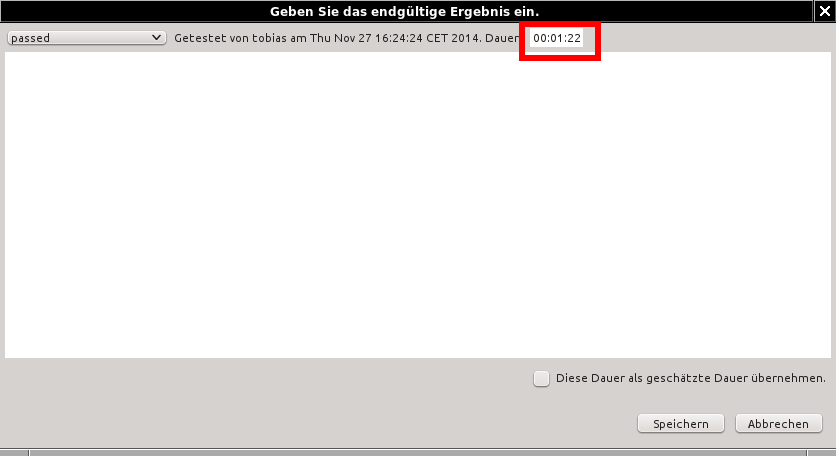
\includegraphics[width=\textwidth]{./BilderAenderungen/endgueltiges-ergebnis-zeit-bearbeitbar-neu.png}
 % endgueltiges-ergebnis-zeit-bearbeitbar.png: 700x456 pixel, 96dpi, 18.52x12.06 cm, bb=0 0 525 342
\end{figure}
Bei der Testfallausführung kann bei der Eingabe des endgültigen Ergebnisses nun die Testzeit nachträglich geändert werden.

\subsection{Bestandene Testfälle in Übersicht deutlich markieren}
\begin{figure}[H]
 \centering
 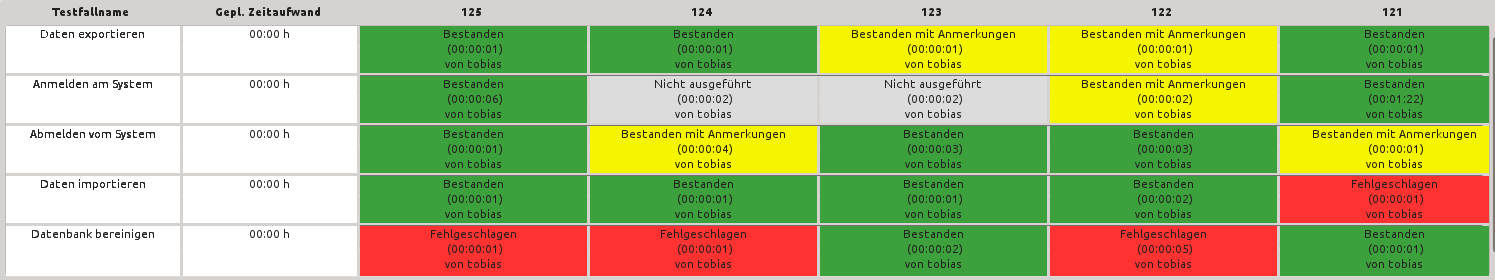
\includegraphics[width=\textwidth]{./BilderAenderungen/uebersicht.png}
 % uebersicht.png: 1495x280 pixel, 96dpi, 39.55x7.41 cm, bb=0 0 1121 210
\end{figure}
Bisher musste für jeden Testfall über eine ganze Zeile hinweg verfolgt werden, was der Status der letzten Ausführung war.
Nun ist die erste Spalte entsprechend dem Status der letzten Ausführung eingefärbt:\\
\begin{figure}[H]
 \centering
 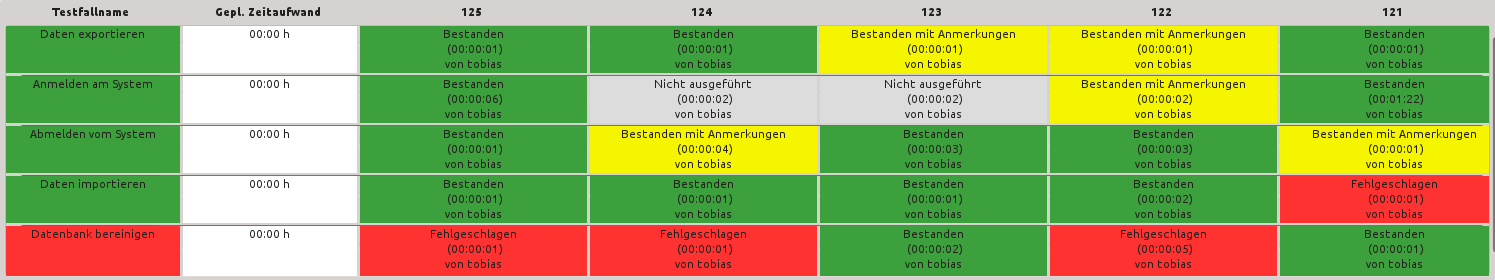
\includegraphics[width=\textwidth]{./BilderAenderungen/uebersicht-neu.png}
 % uebersicht-neu.png: 1495x280 pixel, 96dpi, 39.55x7.41 cm, bb=0 0 1121 210
\end{figure}

\subsection{Benutzeroberfläche vereinfachen durch Ausblendungen}
\begin{figure}[H]
 \centering
 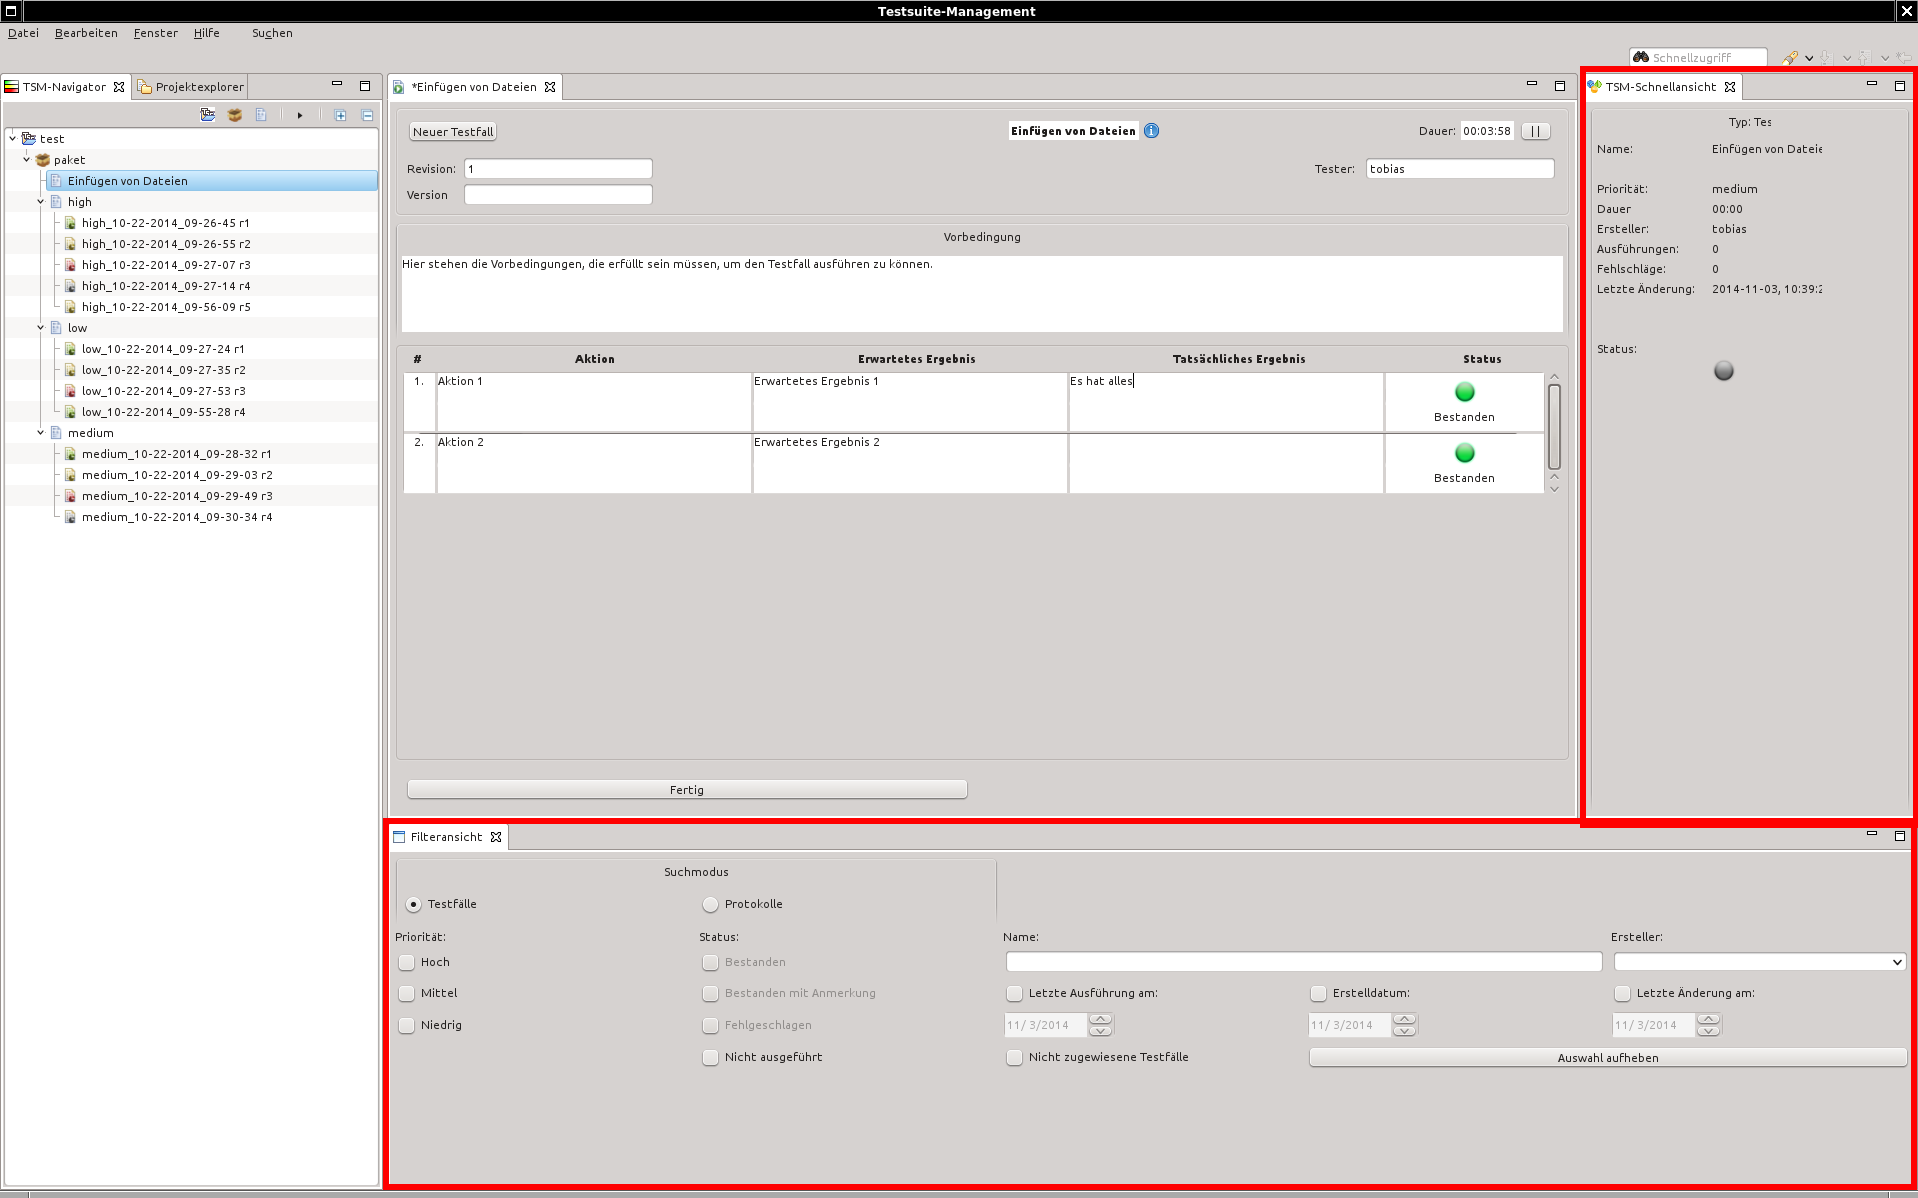
\includegraphics[width=\textwidth]{./BilderAenderungen/ansicht-vereinfachen.png}
 % ansicht-vereinfachen.png: 1918x1198 pixel, 96dpi, 50.74x31.69 cm, bb=0 0 1438 898
\end{figure}
Die Benutzeroberfläche wurde vereinfacht.
Die Schnellansicht und die Filteransicht sind nun im Normalfall nicht sichtbar.
Sie können mittels Klick auf die Schaltflächen \texttt{Filter} und \texttt{Schnellansicht} in der Werkzeugleiste ein- und ausgeblendet werden.

\begin{figure}[H]
 \centering
 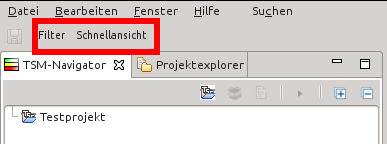
\includegraphics{./BilderAenderungen/filter-schnellansicht-neu.png}
 % filter-schnellansicht-neu.png: 387x144 pixel, 96dpi, 10.24x3.81 cm, bb=0 0 290 108
\end{figure}


\subsection{Speichern-Knopf}
\begin{figure}[H]
 \centering
 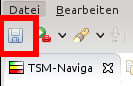
\includegraphics[scale=1.5]{./BilderAenderungen/speichern-knopf.png}
 % speichern-knopf.png: 133x86 pixel, 96dpi, 3.52x2.28 cm, bb=0 0 100 64
\end{figure}
In der Werkzeugleiste ist nun ein Speichern-Knopf vorhanden.

\subsection{Erweitern-Knopf}
\begin{figure}[H]
 \centering
 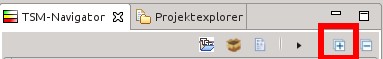
\includegraphics[width=\textwidth]{./BilderAenderungen/erweitern-knopf.png}
 % erweitern-knopf.png: 383x59 pixel, 96dpi, 10.13x1.56 cm, bb=0 0 287 44
\end{figure}
Im TSM-Navigator können nun alle seine Elemente aufgeklappt werden.


\subsection{Handbuch}
Das Handbuch wurde an die neue Version angepasst.

\section{Neue Funktionalität}
\subsection{Anbindung an Versionsverwaltung}
TSM verfügt nun über eine Anbindung an das Versionsverwaltungssystem Subversion.
Zur Einrichtung und Nutzung finden Sie im Handbuch alle nötigen Hinweise.

 
\end{document}

